\section{Simulation}\label{sec:simulation}
\frame{\tableofcontents[currentsection]}

%-------------------------------------------------
\subsection{Simulation Elements}\label{subsec:simulation-elements}

\begin{frame}
    \frametitle{Simulation Elements}
    The aim of th simulation is to determine whether a situated recommendation system may help reduce the waiting time needed to benefit from an attraction.

    \bigskip

    In order to achieve this, two simulations will be developed:
    \begin{enumerate}
        \item \textbf{Random Redirection} reflecting the current system.
        \item \textbf{Recommended Redirection} reflecting the desired system.
    \end{enumerate}

    \bigskip

    The model of the simulation includes:
    \begin{itemize}
        \item A real world map of the Mirabilandia amusement park.
        \item Attractions of many types physically situated on the map.
        \item Visitors able to move towards a specific attraction, chosen with a predefined policy.
    \end{itemize}

\end{frame}
%------------------------------------------------

\subsection{The Simulator}\label{subsec:the-simulator}

\begin{frame}
    \frametitle{The Simulator}
    As for the implementation of the simulation, the \textit{Alchemist Simulator} was used for many reasons:
    \begin{itemize}
        \item It provides a \textit{ready-to-use} simulation environment.
        \item It provides an intuitive graphic user interface.
        \item To contribute to the \textit{research and development} area of the \textit{UniBo DISI}.
    \end{itemize}

    \bigskip

    \begin{center}
        \includegraphics[width=0.5\textwidth]{../img/model}
        \label{fig:model}
    \end{center}

\end{frame}
%------------------------------------------------

\subsection{The Environment}\label{subsec:the-environment}

\begin{frame}
    \frametitle{The Environment}
    The map of Mirabilandia, along with its streets, is provided by \textit{OpenStreetMap}.

    \bigskip

    The deployed entities (Alchemist nodes) are \textbf{visitors} and \textbf{attractions}.
    Visitors are represented by black dots, while attractions are squares of different colors depending on their type (restaurant or ride).

    \bigskip

    Communication happens through attractions that are considered as \textbf{access points} that spread information to their neighbourhood.

\end{frame}

\begin{frame}
    \frametitle{The Environment}

    \begin{center}
        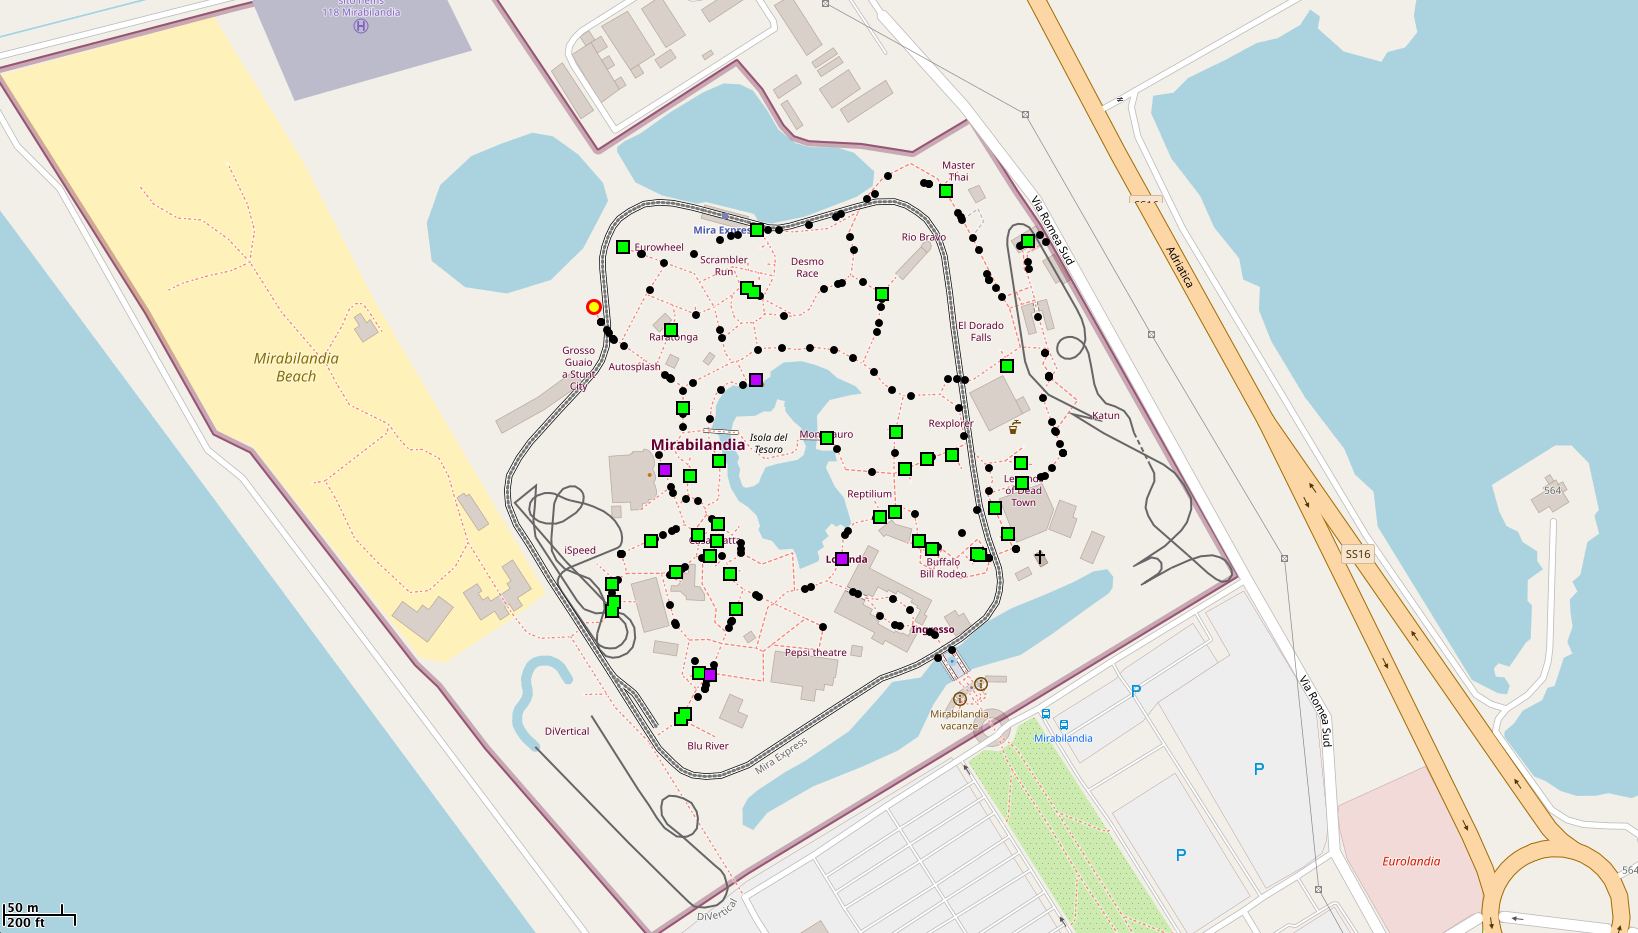
\includegraphics[width=0.5\textwidth]{../img/simulation-screenshot}
        \label{fig:simulation-screenshot}
    \end{center}

\end{frame}
%------------------------------------------------